\begin{center}
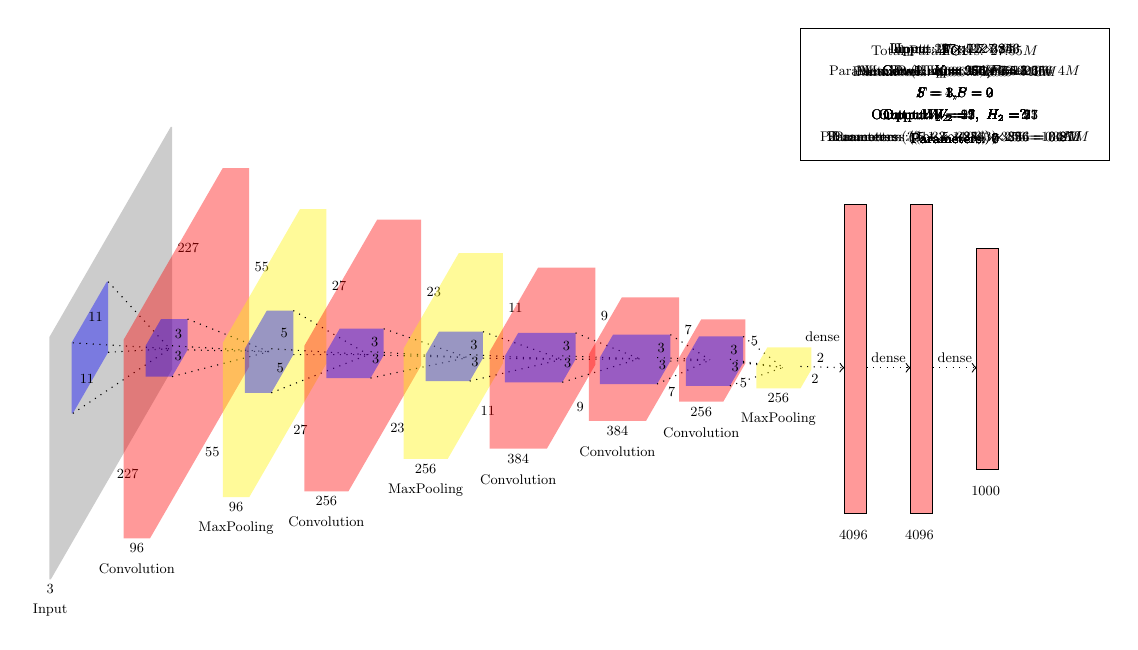
\begin{tikzpicture}[scale=0.56,transform shape]

\pgfsetxvec{\pgfpoint{1cm}{0cm}}
\pgfsetyvec{\pgfpoint{0cm}{1cm}}
\pgfsetzvec{\pgfpoint{-.5cm}{-.866cm}}

\def\cuboid#1#2#3#4#5{
\begin{scope}
\edef\mycolor{#2}
\edef\depth{#3}
\edef\height{#4}
\edef\width{#5}
\draw[black,fill=\mycolor, fill opacity=0.4, text opacity=1] #1 -- ++(-\depth,0,0) -- ++(0,-\height,0) -- ++(\depth,0,0) -- cycle #1 -- ++(0,0,-\width) -- ++(0,-\height,0) -- ++(0,0,\width) -- cycle  #1 -- ++(-\depth,0,0) -- ++(0,0,-\width) -- ++(\depth,0,0) -- cycle;
\end{scope}
}

\def\cuboidlabel#1#2#3#4#5#6#7#8{
\begin{scope}
\edef\mycolor{#2}
\edef\depth{#3}
\edef\height{#4}
\edef\width{#5}
\edef\depthlabel{#6}
\edef\heightlabel{#7}
\edef\widthlabel{#8}
\draw[draw=none,fill=\mycolor, fill opacity=0.4, text opacity=1] #1 -- ++(-\depth,0,0) -- ++(0,-\height,0) -- ++(\depth,0,0) node[black,pos=0.5,below] {\small \depthlabel} -- cycle #1 -- ++(0,0,-\width) -- ++(0,-\height,0) node[black,pos=0.5,right] {\small \heightlabel} -- ++(0,0,\width)  node[black,pos=0.5,below,right] {\small \widthlabel} -- cycle  #1 -- ++(-\depth,0,0) -- ++(0,0,-\width) -- ++(\depth,0,0) -- cycle;
\end{scope}
}

\def\kernel#1#2#3#4#5#6{
\begin{scope}
\edef\mycolor{#2}
\edef\depth{#3}
\edef\height{#4}
\edef\width{#5}
\draw[black,fill=\mycolor, fill opacity=0.4, text opacity=1] #1 -- ++(-\depth,0,0) -- ++(0,-\height,0) -- ++(\depth,0,0) -- cycle #1 -- ++(0,0,-\width) -- ++(0,-\height,0) -- ++(0,0,\width) -- cycle  #1 -- ++(-\depth,0,0) -- ++(0,0,-\width) -- ++(\depth,0,0) -- cycle;

\draw[dotted] #1 -- #6 #1++(0,0,-\width) -- #6 #1++(0,-\height,0) -- #6 #1++(0,-\height,-\width) -- #6;

\end{scope}
}

\def\kernellabel#1#2#3#4#5#6#7#8#9{
%#6 is target pixel
\begin{scope}
\edef\mycolor{#2}
\edef\depth{#3}
\edef\height{#4}
\edef\width{#5}
\edef\depthlabel{#7}
\edef\heightlabel{#8}
\edef\widthlabel{#9}
\draw[draw=none,fill=\mycolor, fill opacity=0.4, text opacity=1] #1 -- ++(-\depth,0,0) -- ++(0,-\height,0) -- ++(\depth,0,0) -- cycle #1 -- ++(0,0,-\width) -- ++(0,-\height,0) node[pos=0.5,left] {\small \heightlabel} -- ++(0,0,\width)  node[pos=0.6,above] {\small \widthlabel} -- cycle  #1 -- ++(-\depth,0,0) -- ++(0,0,-\width) -- ++(\depth,0,0) -- cycle;

\draw[dotted] #1 -- #6 #1++(0,0,-\width) -- #6 #1++(0,-\height,0) -- #6 #1++(0,-\height,-\width) -- #6;

\end{scope}
}

\cuboid{(24,7,0)}{white}{7}{3}{0}{256}{2}{2}

%alexnet
\onslide<1->{
\cuboidlabel{(0,0,0)}{gray}{0.03}{5.5}{5.5}{3}{227}{227}
\node (a) at (-0.015,-6.2,0) {\small Input};
}
\onslide<2->{
\kernellabel{(0,-1,-1)}{blue}{0.03}{1.6}{1.6}{(1.7,-2,-2)}{3}{11}{11}
}
\onslide<2-4>{
\node (a) at (24-7*0.5,7-0.5) {\small Input: $227 \times 227 \times 3$};
\node (a) at (24-7*0.5,7-1) {\small Conv1: $K=96$,$F=11$};
\node (a) at (24-7*0.5,7-1.5) {\small $S=4$,$P=0$};
\onslide<2>{\node (a) at (24-7*0.5,7-2) {\small Output:$W_2=?,\ H_2=?$};}
\onslide<3-4>{\node (a) at (24-7*0.5,7-2) {\small Output:$W_2=55,\ H_2=55$};}
\onslide<2-3>{\node (a) at (24-7*0.5,7-2.5) {\small Parameters: $?$};}
\onslide<4>{\node (a) at (24-7*0.5,7-2.5) {\small Parameters: $(11\times 11 \times 3)\times 96 = 34K$};}
}

\onslide<3->{
\cuboidlabel{(2,-0.5,-0.5)}{red}{0.6}{4.5}{4.5}{96}{55}{55}
\node (a) at (2-0.3,-0.5-4.5-0.7,-0.5) {\small Convolution};
}
\onslide<5->{
\kernellabel{(2,-1.5,-1.5)}{blue}{0.6}{0.7}{0.7}{(3.7,-2.5,-2.5)}{96}{3}{3}
}
%\onslide<4>{
%\node (a) at (2-0.3+1,-6.7,-0.5) {\scriptsize $S=2$,$P=0$};
%\node (a) at (2-0.3+1,-7.2,-0.5) {\scriptsize Parameters: 0};
%}

\onslide<5-7>{
\node (a) at (24-7*0.5,7-1) {\small Max Pool Input: $55 \times 55 \times 96$};
\node (a) at (24-7*0.5,7-1.5) {\small $F=3$,$S=2$};
\onslide<5>{\node (a) at (24-7*0.5,7-2) {\small Output:$W_2=?,\ H_2=?$};}
\onslide<6-7>{\node (a) at (24-7*0.5,7-2) {\small Output:$W_2=27,\ H_2=27$};}
\onslide<5-6>{\node (a) at (24-7*0.5,7-2.5) {\small Parameters: $?$};}
\onslide<7>{\node (a) at (24-7*0.5,7-2.5) {\small Parameters: $0$};}
}


\onslide<6->{
\cuboidlabel{(4,-1,-1)}{yellow}{0.6}{3.5}{3.5}{96}{27}{27}
\node (a) at (4-0.3,-1-3.5-0.7,-1) {\small MaxPooling};
}
\onslide<8->{
\kernellabel{(4,-2,-2)}{blue}{0.6}{1}{1}{(5.7,-3,-3)}{96}{5}{5}
}
%\onslide<6>{
%\node (a) at (4-0.3+1,-6.7,-1) {\scriptsize $S=1$,$P=0$};
%\node (a) at (4-0.3+1,-7.2,-1) {\scriptsize Parameters: $(5\times 5 \times 96)\times 256 = K$};
%}

\onslide<8-10>{
\node (a) at (24-7*0.5,7-0.5) {\small Input: $27 \times 27 \times 96$};
\node (a) at (24-7*0.5,7-1) {\small Conv1: $K=256$,$F=5$};
\node (a) at (24-7*0.5,7-1.5) {\small $S=1$,$P=0$};
\onslide<8>{\node (a) at (24-7*0.5,7-2) {\small Output:$W_2=?,\ H_2=?$};}
\onslide<9-10>{\node (a) at (24-7*0.5,7-2) {\small Output:$W_2=23,\ H_2=23$};}
\onslide<8-9>{\node (a) at (24-7*0.5,7-2.5) {\small Parameters: $?$};}
\onslide<10>{\node (a) at (24-7*0.5,7-2.5) {\small Parameters: $(5\times 5 \times 96)\times 256=0.6M$};}
}

\onslide<9->{
\cuboidlabel{(6,-1.5,-1.5)}{red}{1}{3.3}{3.3}{256}{23}{23}
\node (a) at (6-0.5,-1.5-3.3-0.7,-1.5) {\small Convolution};
}
\onslide<11->{
\kernellabel{(6,-2.5,-2.5)}{blue}{1}{0.6}{0.6}{(7.7,-3.5,-3.5)}{256}{3}{3}
}
%\onslide<8>{
%\node (a) at (6-0.5+1,-6.7,-1.5) {\scriptsize $S=2$,$P=0$};
%\node (a) at (6-0.5+1,-7.2,-1.5) {\scriptsize Parameters: 0};
%}

\onslide<11-13>{
\node (a) at (24-7*0.5,7-1) {\small Max Pool Input: $23 \times 23 \times 256$};
\node (a) at (24-7*0.5,7-1.5) {\small $F=3$,$S=2$};
\onslide<11>{\node (a) at (24-7*0.5,7-2) {\small Output:$W_2=?,\ H_2=?$};}
\onslide<12-13>{\node (a) at (24-7*0.5,7-2) {\small Output:$W_2=11,\ H_2=11$};}
\onslide<11-12>{\node (a) at (24-7*0.5,7-2.5) {\small Parameters: $?$};}
\onslide<13>{\node (a) at (24-7*0.5,7-2.5) {\small Parameters: $0$};}
}


\onslide<12->{
\cuboidlabel{(8,-2,-2)}{yellow}{1}{2.5}{2.5}{256}{11}{11}
\node (a) at (8-0.5,-2-2.5-0.7,-2) {\small MaxPooling};
}
\onslide<14->{
\kernellabel{(8,-3,-3)}{blue}{1}{0.6}{0.6}{(9.7,-3.8,-3.8)}{256}{3}{3}
}
%\onslide<10>{
%\node (a) at (8-0.5+1,-6.7,-2) {\scriptsize $S=1$,$P=0$};
%\node (a) at (8-0.5+1,-7.2,-2) {\scriptsize Parameters: $(3\times 3 \times 256)\times 384 = K$};
%}
\onslide<14-16>{
\node (a) at (24-7*0.5,7-0.5) {\small Input: $11 \times 11 \times 256$};
\node (a) at (24-7*0.5,7-1) {\small Conv1: $K=384$,$F=3$};
\node (a) at (24-7*0.5,7-1.5) {\small $S=1$,$P=0$};
\onslide<14>{\node (a) at (24-7*0.5,7-2) {\small Output:$W_2=?,\ H_2=?$};}
\onslide<15-16>{\node (a) at (24-7*0.5,7-2) {\small Output:$W_2=9,\ H_2=9$};}
\onslide<14-15>{\node (a) at (24-7*0.5,7-2.5) {\small Parameters: $?$};}
\onslide<16>{\node (a) at (24-7*0.5,7-2.5) {\small Parameters: $(3\times 3 \times 256)\times 384=0.8M$};}
}

\onslide<15->{
\cuboidlabel{(10,-2.5,-2.5)}{red}{1.3}{2.2}{2.2}{384}{9}{9}
\node (a) at (10-0.65,-2.5-2.2-0.7,-2.5) {\small Convolution};
}
\onslide<17->{
\kernellabel{(10,-3.2,-3.2)}{blue}{1.3}{0.6}{0.6}{(11.5,-3.7,-3.7)}{384}{3}{3}
}
%\onslide<12>{
%\node (a) at (10-0.65+1,-6.7,-2.5) {\scriptsize $S=1$,$P=0$};
%\node (a) at (10-0.65+1,-7.2,-2.5) {\scriptsize Parameters: $(3\times 3 \times 384)\times 384 = K$};
%}
\onslide<17-19>{
\node (a) at (24-7*0.5,7-0.5) {\small Input: $9 \times 9 \times 384$};
\node (a) at (24-7*0.5,7-1) {\small Conv1: $K=384$,$F=3$};
\node (a) at (24-7*0.5,7-1.5) {\small $S=1$,$P=0$};
\onslide<17>{\node (a) at (24-7*0.5,7-2) {\small Output:$W_2=?,\ H_2=?$};}
\onslide<18-19>{\node (a) at (24-7*0.5,7-2) {\small Output:$W_2=7,\ H_2=7$};}
\onslide<17-18>{\node (a) at (24-7*0.5,7-2.5) {\small Parameters: $?$};}
\onslide<19>{\node (a) at (24-7*0.5,7-2.5) {\small Parameters:  $(3\times 3 \times 384)\times 384=1.327M$};}
}


\onslide<18->{
\cuboidlabel{(12,-3,-3)}{red}{1.3}{1.5}{1.5}{384}{7}{7}
\node (a) at (12-0.65,-3-1.5-0.7,-3) {\small Convolution};
}
\onslide<20->{
\kernellabel{(12,-3.5,-3.5)}{blue}{1.3}{0.6}{0.6}{(13,-3.9,-3.9)}{384}{3}{3}
}
%\onslide<14>{
%\node (a) at (12-0.65+1,-6.7,-3) {\scriptsize $S=1$,$P=0$};
%\node (a) at (12-0.65+1,-7.2,-3) {\scriptsize Parameters: $(3\times 3 \times 384)\times 256 = K$};
%}
\onslide<20-22>{
\node (a) at (24-7*0.5,7-0.5) {\small Input: $7 \times 7 \times 384$};
\node (a) at (24-7*0.5,7-1) {\small Conv1: $K=256$,$F=3$};
\node (a) at (24-7*0.5,7-1.5) {\small $S=1$,$P=0$};

\onslide<20>{\node (a) at (24-7*0.5,7-2) {\small Output:$W_2=?,\ H_2=?$};}
\onslide<21-22>{\node (a) at (24-7*0.5,7-2) {\small Output:$W_2=5,\ H_2=5$};}
\onslide<20-21>{\node (a) at (24-7*0.5,7-2.5) {\small Parameters: $?$};}
\onslide<22>{\node (a) at (24-7*0.5,7-2.5) {\small Parameters:  $(3\times 3 \times 384)\times 256=0.8M$};}
}

\onslide<21->{
\cuboidlabel{(13.5,-3.5,-3.5)}{red}{1}{1}{1}{256}{5}{5}
\node (a) at (13.5-0.5,-3.5-1-0.7,-3.5) {\small Convolution};
}
\onslide<23->{
\kernellabel{(13.5,-3.8,-3.8)}{blue}{1}{0.6}{0.6}{(14,-5.2,-5.2)}{256}{3}{3}
}
%\onslide<16>{
%\node (a) at (13.5-0.5+1,-6.7,-3.5) {\scriptsize $S=2$,$P=0$};
%\node (a) at (13.5-0.5+1,-7.2,-3.5) {\scriptsize Parameters: 0};
%}
\onslide<23-25>{
\node (a) at (24-7*0.5,7-1) {\small Max Pool Input: $5 \times 5 \times 256$};
\node (a) at (24-7*0.5,7-1.5) {\small $F=3$,$S=2$};
\onslide<23>{\node (a) at (24-7*0.5,7-2) {\small Output:$W_2=?,\ H_2=?$};}
\onslide<24-25>{\node (a) at (24-7*0.5,7-2) {\small Output:$W_2=2,\ H_2=2$};}
\onslide<23-24>{\node (a) at (24-7*0.5,7-2.5) {\small Parameters: $?$};}
\onslide<25>{\node (a) at (24-7*0.5,7-2.5) {\small Parameters:  $0$};}
}


\onslide<24->{
\cuboidlabel{(14.5,-5,-5)}{yellow}{1}{0.5}{0.5}{256}{2}{2}
\node (a) at (14.5-0.5,-5-0.5-0.7,-5) {\small MaxPooling};
}

\onslide<26>{
\node (a) at (24-7*0.5,7-0.5) {\small FC1};
\node (a) at (24-7*0.5,7-1) {\small Parameters: $(2\times 2 \times 256)\times 4096 = 4M$};
}

\onslide<26->{
\draw[dotted,->] (14.5,-5,-5) -- (18,-0.7,0);
\node (a) at (17.5,0,0) {\small dense};
\cuboid{(18.5,3,0)}{red}{0.5}{7}{0}{256}{2}{2}
\node (a) at (18.2,-4.5,0) {\small 4096};
}

\onslide<27>{
\node (a) at (24-7*0.5,7-0.5) {\small FC1};
\node (a) at (24-7*0.5,7-1) {\small Parameters: $4096 \times 4096 = 16M$};
}

\onslide<27->{
\draw[dotted,->] (18.5,-0.7,0) -- (19+0.5,-0.7,0) node[pos=0.5,above] {\small dense};
\cuboid{(19.5+0.5,3,0)}{red}{0.5}{7}{0}{256}{2}{2}
\node (a) at (19.2+0.5,-4.5,0) {\small 4096};
}

\onslide<28->{
\draw[dotted,->] (19.5+0.5,-0.7,0) -- (20+1,-0.7,0) node[pos=0.5,above] {\small dense};
\cuboid{(20.5+1,2,0)}{red}{0.5}{5}{0}{256}{2}{2}
\node (a) at (20.2+1,-3.5,0) {\small 1000};
}


\onslide<28>{
\node (a) at (24-7*0.5,7-0.5) {\small FC1};
\node (a) at (24-7*0.5,7-1) {\small Parameters: $4096 \times 1000 = 4M$};
}
\onslide<29>{
\node (a) at (24-7*0.5,7-0.5) {\small Total Parameters: $27.55M$};
}





\end{tikzpicture}
\end{center}

